

\documentclass[twoside,titlepage]{article}


\usepackage{animate}
\usepackage{amssymb}
\usepackage{amsmath}
\usepackage{graphicx}
\usepackage{easylist}
\usepackage{fancyhdr}
\usepackage{enumerate}
\usepackage{nameref}
\usepackage{titling}
\usepackage{diagmac2}
\usepackage{forloop}
\include{tikz}
\usetikzlibrary{mindmap}
\usepackage{subfigure}
\usepackage{ulem}


\pagestyle{fancyplain}
\fancyhf{}
\fancyhf[FLO,FRE]{\thepage}
\fancyhead[RE,LO]{\thesection.\currentname.}

\renewcommand{\abstractname}{}
\renewcommand{\thesection}{\thepart \Alph{section}}
\renewcommand{\theenumi}{\thesection\arabic{enumi}}
\renewcommand{\theenumii}{\theenumi.\arabic{enumii}}

\makeatletter
\newcommand*{\currentname}{\@currentlabelname}
\makeatother


\begin{document}

 








\title{Relationship Agreement between Danielle Jackson and Samuel Carter}
\author{ Danielle Jackson, Ph.D \and Lieutenant Colonel Samuel Carter }
\date{20/3/2013}
\maketitle
 \begin{abstract}
This Document Dictates, the terms, conditions and agreements, between both parties for what they have decided  
each party must do,or not do, owe, or is owing of them.
 \end{abstract}




 \tableofcontents

 
 \section{Relationship Rules}
\begin{enumerate}
  \item \sout{Neither party may kiss one another. Kissing is defined as the touching of lips. The touching of one set of lips to another
   body part is allowed unless it breaks another following rule.} Voided as of 27/3/13
  \item Touching between the parties is limited to hugs. A hug is defined as the wrapping of arms around one and other, and
   must occur once per meeting between Sam and Danielle.
   \\\textbf{\emph{Amendment}}
  \begin{enumerate}
    \item Samuel is permitted to touch Danielle in the breast area, and the buttocks region, while both parties are in private. 
  \end{enumerate}
  \item  No Item or Favour owed, may be used to force either Sam or Danielle into forfeiting or losing a Wager, or dare. 
  Hours of time may not be used to force a party into doing something they are currently unwilling to do. 
  \\ \textbf{\emph{Amendment}}
  \begin{enumerate}
    \item However a Dare may be used in conjunction with an item or favour, if it does not adversely affect the intent 
    of the reward, or the goal set within the dare.
    \item  If it does change the intent. A new Dare must be made, to be completed at another time
  \end{enumerate}
  \item If copulation in the shower is to occur it should be done early in the wash cycle as to minimise, the loss of hot water.
  \item Copulation in the bath should be discouraged as to minimise water spillage, but groping and touching should be encouraged.
  \item Copulation in the pool is to be expected, assuming cover of darkness but limited due to chlorine
  \item When a Challenge/Dare is complete it is Crossed out, but may be reintroduced with an amendment at a later date.
  \item On Tuesday and Thursday, should Danielle or Sam attempt to communicate with each other via any Online means, 
  An hour of time will be given to the other. This does not include, After Hours Ramblings,Questions relating to Work, 
  the need for Danielle or Sam to destress and thus needing the other, Or goodnights if they extend from Monday or Wednesday 
  into the early hours of Tuesday or Thursday.
  \item A minimum of an hour must be given to the other party that you will be coming over, if you expect their place to be tidy,
  otherwise you have no grounds to complain.
  \item 
\end{enumerate}
 




 

 

 

 \newpage
 \section{Miscellaneous Rules}

 \begin{enumerate}
   \item Do not talk about the //
   \item DO NOT talk about the //
   \item If you must talk about the //, it is the  `slash' and should be addressed as any other fanfiction we mutually read.
   \item When talking about the //, Pseudonyms will be used, no exceptions.
   \item When referring to a Rule You cannot call it a Rule. No exceptions.
   \item If you must refer to a Rule refer to it by Code �B06� No exceptions.
   \item If you wish to invoke an Owe While in the presence of another, make obscure reference only Or DON�T.
   \item Punishment for Breaking rules 1-7 Results in loss of rights to ask for sex for a 48 Hour Period.
   \\ \textbf{\emph{Amendment}}
  \begin{enumerate}
    \item This does not preclude sex, simply means it  MUST not be initiated by the one being punished.
    \item Rights to invoke Owes of a sexual nature are revoked for the day as well
    \item Dares in which are to be completed in the 24 hour period  because of circumstances are unable to be completed, 
    The 48 hours may be shifted forward till after the dare/challenge is completed.
  \end{enumerate}
   \item Should the printed copy of this Document Be found by an outsider due to the negligence of either Danielle or Sam 
   then they must Submit themselves to do something outside their comfort zone emotionally in front of the peers of the either party.
   \item McShep is the OTP. End of Story.
   \item All apples must be consumed by slicing into the apple with a knife, cutting it into pieces.
   \item Anything you say can and will be used against you.
   \item Anything you do can and will be used against you, so you do it again.
   \setcounter{enumi}{33}
   \item If its going to be done, its on the list
   \item If its not on the list it will be added
   \setcounter{enumi}{98}
   \item Sam and Danielle agree that they are both open to degrees of sexual experimentation assuming 
   both parties are on board and does not impair physical, mental or emotional wellbeing. 
   \\ \textbf{\emph{Amendment}}
  \begin{enumerate}
    \item If an hour passes unable to decide what to do, the defaulted choice is sexual experimentation.
    \item  If an hour has passed with no decision being made, and Danielle and Sam are in a social outing 
    and unable to perform rule B99.1, the two must default to Sex-ting each other. 
  \end{enumerate}
 \end{enumerate}
 
 \cleardoublepage
 
 \section{Situational Rules}

 \begin{enumerate}
   \item Should one party be given a ring of immense power that must be destroyed by completing a long journey, they agree to traverse the path together, 
   and kill any creepy half human things that attempt to help them, and carry the partner should they need it.
	\\ \textbf{\emph{Amendment}}
  	\begin{enumerate}
    	\item Simply call the flying Eagles
    	\item Do not hesitate to destroy ring in fires
    	\item Use Elvish as frequently as plot allows
  	\end{enumerate}
  	
   	\item Should either party find a Book in which if a name is written, that person should die, We will both work together 
   to become a seemless killing machine with ourselves placed as gods, and work together to play Xantatos Chess.
   \item If awaken to find ourself�s within confines of faerytale realm, Danielle gets to be the conquering Heroine who saves Sam from peril.
   \item Should either party decide that Meat is no longer required and thus turn vegan or vegetarian, the other party will proceed to slap 
   them with Cow and Pig or force feed them curry.
   \item When one party is studying/working/concentrating, the other party agrees to leave them alone and not attempt to seduce them with sex.
   \\ \textbf{\emph{Amendment}}
  \begin{enumerate}
    \item Should the rule be broken, the other must give a full body massage to the Worker.
  \end{enumerate}
  \item Should Danielle Be captured by a Giant Mutant Turtle beast, And Sam goes on an adventure, surpassing many challenges, Danielle will 
  leave a note on the front of the Castle she is actually in, or scream as to give Sam an indication whether or not to fight his way through the castle.
  \item 
  \item If either party gains the Ability to fly or teleport through Super Powers, Magic, or otherwise, they agree to fly/teleport the other as both a means
   of travel, and as a joyful activity.
   \item Should Either party Gain a Super Powers, or magic via any means they will endeavour to empower the other with complementing or contrasting abilities 
   so as to form a Super Hero Team.
   \\ \textbf{\emph{Amendment}}
  \begin{enumerate}
    \item Costumes should be inventive, not derivative and not involve external underwear,spandex of any kind or leather pants.
    \item NO CAPES
    \item If Children are in the future, we shall ensure that the powers are genetic, or else given to them at an early age as to teach them to handle them.
   \end{enumerate} 
  
  \item Should either of us discover a Fob watch, we gift it to the other person as to let them determine the calibre of TimeLord/Lady
  \\ \textbf{\emph{Amendment}}
  \begin{enumerate}
    \item If it is discerned that the timelord is malicious, we hunt for Tardis
    \item If Timelord is nice, then we agree to open, with promise of travelling universe together. 
  \end{enumerate}
  \item In the situation that a Condom cannot be found, then...
  \item Should Either become an Evil Genius or Overlord, they will follow the Evil Overlord list, 
  as they are logical and will help them enslave the populations. 
  \item If either acquires the technology to create nanobots to shape the universe for their own gain, 
  they agree that they will keep with the terms agreed upon originally discussed.
  \setcounter{enumi}{30}
  \item If either of us invents time travel we will ensure to make the Vehicle in a which we traverse time and space to either be an 
  infinitely large blue police box, or a Delorean.
  \\ \textbf{\emph{Amendment}}
  \begin{enumerate}
    \item Sex in either is fine, and encouraged.
  \end{enumerate}
  
  \item Should either party Become a Zombie, with an almost nil chance of a antivirus being developed Then Depending 
  on nature of Zombies:
   \\ \textbf{\emph{Amendment}}
  \begin{itemize}
    \item  For Intelligent zombies that posses brain capacity and are simply the undead with a craving for brain -
     we bite the other and gain immortality.
     \item For mindless meandering zombies - shoot first cry later, however the method of death must be enacted by 
     the non zombie party, assuming it is possible given circumstances.  
  \end{itemize}
  
  \item  In the event both Danielle and Sam switch bodies, They agree to teach the other everything they can about their mannerisms and persona, 
  as well as doing all things sexual to both themselves and their partner, and going out experiencing everything they can about the 
  other person�s life.  
  \item In the Event of a Gender Swap of both parties it is agreed that they will attempt to  progress along the linear progression of 
  �bases� until such a point as awkwardness overcomes pleasure. They will also a session of Cosplaying assuming costumes fit, or the 
  genderswap lasts a time that costumes can be bought.
  \\ \textbf{\emph{Amendment}}
  \begin{enumerate}
    \item In the case of only Danielle being Gender swapped it is agreed that they will attend a Strip club together as gentlemen, 
    drink scotch while puffing cigars, and also attempt to conduct a Devil�s threeway. There will also be a session of mutual 
    masterbation along with an attempted 69.
    \item In the case of only Sam being Gender swapped we have a �girls day out� and then get dressed up and go clubbing, afterwhich
     a session of Lesbian Sex, where Danielle performs cunninglingus on Sam.
  \end{enumerate}
  \item In a situation where one party is covered in whipped cream, or any other condiment of appeal, for the sensation
   of sexual pleasure, the other is duty bound to lick it all off.
  \item If health does not permit any form of contact between the pair, it is agreed that sex-ting via means of SMS messaging, 
  Skype voice/video or text chat or facebook text chat is to be employed until such time that the sick is nursed back to 
  health with care and affection. 
  \item Oral Pleasure while either Danielle or Sam are driving while may seem like a good idea on paper will never be put into practice
  \\ \textbf{\emph{Amendment}}
  \begin{enumerate}
    \item This does not mean that a simulated experience cannot occur, but this shall never occur while the vehicle is ``Turned on''. 
  \end{enumerate}
  
  \item In the event of accidental incident with time travel, it is agreed that Sam protects Danielle with the benefits of 
  masculinity, while Danielle attempts to understand period and use knowledge to benefit both. 
  \item If Sam or Danielle rise to the ranks in the underworld or heaven, assist their human to rise with the, assuring 
  them a decent place in underworld.
  \item Should One party make a deal with Satan thus leading the other on a Quest through the Inferno in an effort to save 
  the other from satan's grasp, it is agreed that the angelic party who has been taken by satan, will help through Divine 
  intervention wherever plot allows it, and will ensure a spot in the 1st Sphere of Paradiso.
  \item Should either party be taken by an incubi or succubi, it is agreed that this is not a form of cheating and both parties 
  will attempt to slay the foul creature and raise bastard half satanic children as their own.   
  \item In the event of parties being sucked into science fiction novel, both parties will proceed as quickly as possibly to acquire towels.
  \item In the case that someone learns about the //  we either employ blackmail or Physical force.
  \item We agree we will never be apart of the people that go to the special hell reserved for child molesters and people who talk in the cinema.
  \\ \textbf{\emph{Amendment}}
  \begin{enumerate}
    \item Physical force may include but is not limited to: 
    \begin{itemize}
      	\item  Murder
		\item  Stabbing
		\item  Retinas burnt out with Giant Laser
		\item  Frontal Lobe scooped out
		\item  Hands cut off
		\item  Crucifixion
		\item  light tapping on the shoulder
		\item  Chinese Water torture  
    \end{itemize}
  \end{enumerate}
  \item If either party is upgraded, then we agree to contain party and attempt to transplant brain.
  \item Should the ability to clone oneselves become commonly avaliable or developed by either party, then the Clones are restricted to a maximum of 5,
   and are welcome to be used as �sex toys�. 
   \item In the event of a crossover or transvergence with Parallel universe, we agree to meet alternate forms of self and determine from there 
   possibility of a threesome or greater. 
  \setcounter{enumi}{52}
  \item Should it be discovered that either Sam or Danielle are actually creatures inhabiting a body, 
  as per the conventions of a non-harmful symbiotic relationship, it is agreed that they will not judge the other or 
  attempt to enslave humans throughout the galaxy, or perpetuate hybrid race with their larva in navel cavity.
  \item Should either party have the genes of a long dead Hyper intelligent Race, we agree to take the other to the 
  long lost city, should we be invited to go on the expedition.
  \item Should either party ascend, particularly Danielle, it is agreed that the newly ascended will visit and attempt 
  to help the ascension process, but not before sharing themselves with the other.
  \item In the event that both of our families start a long feud, and we are caught in the middle of it, we agree we will 
  send messages before doing anything drastic.
  \setcounter{enumi}{68}
  \item If a situation arises such that both Sam and Danielle are wanting to please the other Orally and neither wishes 
  to wait then both shall perform the oral in the sexual position 69.
  \setcounter{enumi}{70}
  \item In any given disagreement, pausing and resuming are always an option, with no repercussions for doing so, as well 
  as requesting for a breather to gather thoughts and speak calmly.
  \item In the event of an altercation between Sam and Danielle, then they both agree that at the end of the fight, make up sex will ensue.
  \\ \textbf{\emph{Amendment}}
  \begin{enumerate}
    \item If the fight is about sex, this is probably a bad idea, and some other form of tension alleviating activity should be undertaken as to 
    reinforce the finality of the particular altercation
  \end{enumerate}
 \end{enumerate}

 \cleardoublepage
 

 

 \section{Owing}
 It is agreed upon that In regards to Hours that the equation
 \large
 \begin{align}
 \text{Hours} &= \frac{22(42\phi)+150\mu + 60\eta}{60}\\
 &= \frac{924}{60}\phi + \frac{150}{60}\mu + \frac{60}{60}\eta\\
 &= \frac{77}{5}\phi + \frac{5}{2}\mu + \eta\\\nonumber
  \text{where}\\ \nonumber
 \phi &=  \text{Number of Seasons Owed}\\\nonumber
 \mu &=  \text{Number of Movies Owed}\\\nonumber
 \eta &=  \text{Number of Extra Hours Owed}
 \end{align}
 
 

  
 \normalsize
 \subsection{Danielle}

 \begin{itemize}
   \item Danielle, has 5 Seasons (77 Hours) of Sam's time to do with as she wishes.\\
    \begin{tabular}{r|rrr|l|r}
 		Date&Season&Movies&Extra&Change&Total\\
 		\hline
 		10/3/2013&+5&&&+77& 77\\
 		\hline
 		\hline
 		Total&5&0&0&&77
 	\end{tabular}
   \item Free Pass To do as Danielle pleases.
   \item The Power to Dictate the clothing choice, for Sam, on any singular day
   \item The choice of 2 Fan Fictions in which Sam must himself read.
   \item The decision for which book, from which chapter, must Sam read aloud.
 \end{itemize} 


 

   \subsection{Samuel}
   \begin{itemize}
     \item Samuel has 6 Seasons, 5 Movies and 2 Hour (107 Hours) of Danielle's time to do with as he wishes.\\
     \begin{tabular}{r|rrr|l||r}
 		Date&Season&Movies&Extra&Change&Total\\
 		\hline
 		10/3/2013&+5&+3	&	&+85	&85 \\
 		16/3/2013&+1&+2	&	&+21	&105\\
 		19/3/2013&	&	&+1	&+1		&106\\
 		21/3/2013&	&	&+1	&+1		&107\\
 		\hline
 		\hline
 		Total&6&5&2&&107
 	\end{tabular}
     \item Sam has the duty to complete the task of combining sex and chocolate.
     \item An Hour of Danielle's time to do with it as he will, or else substitute it for cake.
     \item A free pass to do with her as his every desire commands
     \item The quest to acquire something Danielle can not give.
     \item The Power to Dictate the clothing choice, for Sam, on any singular day as Punishment against
     \item Sam may dictate at any single time in which Danielle must oblige and supply a full body massage.
     \item At a later date, Danielle must determine how she will "Sell herself out for her research".
     \item A Creative Mathematical Themed Idea to be determined.
   \end{itemize}
    
 \cleardoublepage
 
 \section{Wagers}
 \subsection{Oral Challenge:}
 \begin{samepage}
Take a photo Every 30 seconds, One Person Must Retain Composure, while the other proceeds to give Oral to them, 
out of sight of the camera.\\
  \indent $\sim$ \hspace{5mm} Danielle: Sam must stay out of sight underneath Danielle's hoop dress, while pleasuring 
  her to the best of his abilities using all available utilities, while she must
  act as if there is no activity that is 'twixt at her nethers'.\\
 \indent  $\sim$ \hspace{5mm}Sam: Danielle must stay hidden underneath a desk or similar performing whatever ministrations using 
  whatever pleases her to pleasure him, while he attempts not to blow his cover.\\

 
  For each individual photograph in which either party is visibly pleasuring or being pleasured, will provide the other 
  with an hour of your time in which to use freely.
 \end{samepage}

 \subsection{Can't Touch This}
\begin{samepage}
   \indent $\sim$ Until the time of November 9th, neither party may under any circumstances kiss the other. Danielle is 
   unable to touch Sam in any way, directly or indirectly, which could be interpreted as sexual. Sam on the other hand is
    allowed to touch at both the breast and butt area, but may not progress further. \\
    \textit{ Violations of these orders will result in: } 
    \begin{itemize}
      \item The other party being allowed the same opportunity you stole.
      \item A greater than five hundred word porn story containing only both parties.
      \item In the future at a later specified time, the offender will have to follow the innocent,
      around the house naked until such time as the innocent says otherwise or company arrives.
      \item The offender will also have to cook a dinner meal, as well as hand cook a dessert to
       accompany the food.  
    \end{itemize}
\end{samepage}
 

\subsection{Who's' on first} 
\begin{samepage}
   \indent $\sim$ When the time comes that Sam and Danielle eventually copulate, the bed in which the coitus occurred, 
   will be deemed loser, and the other will be given 5 Hours to use at their discretion to have coitus in the losers bed.
\end{samepage}
 

 \subsection{A Song of Desire and Entice (Game of moans)}
\begin{samepage}
   \indent $\sim$ During the viewing of HBO's Game of Thrones, at every sex scene at the end of the scene,
    the show will be paused, and both parties will attempt to bring the other to orgasm.  
    The show will resume when either party has orgasmed. The loser is the first person to desire not to copulate
     but instead return to viewing the show. At that time the winner will receive the amount of hours equaling the total 
     number of episodes watched.

 

 \subsection{Riding on empty} 

   \indent $\sim$ On a day agreed to by both parties, Danielle will attempt to copulate with Sam until  
     such a point that Sam is no longer able to produce an orgasm, or Danielle backs out.  
     The loser will have to give a full body massage to the victor to rub away the pain of 
     coitus. 
\end{samepage}
 

 \subsection{Sex-ting in plain sight}  
\begin{samepage}
  \indent $\sim$ As in rule B99.2 after an hour of nothing but socializing in a group, both parties must  
     sext one and other, assuming the technology is available to do so. Both parties must attempt to hide the fact from the group, 
     that Danielle and Sam are sex-ting one and other. \\
     \indent $\sim$ \hspace{5mm} If either party is caught sex-ting the other, then they are defined as the loser.
       Being caught is defined as being the person on the receiving end of a sext when it is  
       brought to the attention of the group or a subset of.\\ 
     \indent $\sim$ \hspace{5mm} The loser must suffer sensory deprived coitus. A blind fold and earplugs will be 
       employed, and the losing part must not make a noise or touch the winner at all in any way shape or form. 
\end{samepage}
\subsection{Ready Set Blow}
\begin{samepage}
\indent $\sim$ After the prescribed period in which copulation cannot occur, a day will be prescribed in which both 
	Danielle and Sam having not been pleasured for over 24 Hours will attempt this dare. \\
	In this dare both parties will race, predominately through the use of oral techniques to pleasure the other party. 
	This pleasure will occur in a sideways 69 Position, as to give no party leverage over the other \\
	\indent $\sim$ \hspace{5mm} This does not mean that oral techniques be the only techniques employed, but a majority stakehold
	in the pleasure caused.
	The winners is defined as the party who first caused a climax. The winner will recieve A complimentary Season worth of time,
	Along with the ability to recieve Oral pleasure in 5 Unique Locations, excluding the bedroom.
	The loser will recieve a Movies worth of time, along with being finished of the impending climax, for efforts applied
	
\end{samepage}
 \cleardoublepage
 
 

 \section{Dares}

 \renewcommand{\theenumi}{\thesubsection.\arabic{enumi}}

   \subsection{Danielle Dares Sam}

\begin{enumerate}
\item  To stay up and watch the sun to rise with her and kiss her the moment its above the horizon.

\item  To go 2 Hours without making an innuendo, and if he manages to achieve such a feat, will receive fellatio.

\item  To meet her at an establishment pretending not to know her, and attempt to pick her up.

\item  To have a physical Poke war. 

\item  To dress in fitting historical costuming (Toga, Bulla, etc.) and read to her a translation of her favourite poems.  Assuming she can hold out  jumping on him, special reward ensues - must be completed to find out.  hehe 

\item  To sleep with her in her car, preferably during heavy rain (insert `very wet' joke here) 

\item To perform Cunnilingus, after consuming ananas Juice.

\item To To Allow her to lick Tabasco Sauce off of him.

\item To Allow her to lick wasabi off of him.

\end{enumerate}

 

  \subsection{Sam Dares Danielle:}

\begin{enumerate}
\item  To sleep with him with Dynamite by Taio Cruz, playing in background .

\item  To go 2 Hours without Making any reference to history, and if she manages such a feet of the calibre of the labours of Hercules, will receive Cunnilingus. 

\item  To spend all possible time in a day With no clothes on

\item  To awaken Samuel via means of Fellatio.

\item  To Skinny-dip along with Sam in her pool.

\item  To wear her skirt 3 inches above her knee for a single day.

\item  To Do activities in Her car with Sam so that the windows fog, to a point where it is impossible to see from the outside in or the inside out.

\item  To Kiss him in the rain.

\item To attempt an underwater blowjob.

\end{enumerate}

 \cleardoublepage
 
\Section{One True \underline{~~~~~~~~~~}}
\\

\begin{tabular}{c| c|c}
1&\multicolumn{2}{ c }{Slash Pairing}\\ \hline
&M/F  &  \\
&M/M  &  \\
&F/F  &  \\
\hline
2&\multicolumn{2}{ c }{Position}\\ \hline
&Him  &  \\
&Her  &  \\
&Both &  \\
\hline
3& \multicolumn{2}{ c }{TV Show}\\ \hline
&Firefly & Jayne/Hat\\
\hline
4& \multicolumn{2}{ c }{Movie}\\ \hline
\hline
5& \multicolumn{2}{ c }{Book}\\ \hline
\hline
6& \multicolumn{2}{ c }{}\\ \hline
\end{tabular}


 \cleardoublepage
 \section{Lists and Figures}
\label{sec:ListFigures}



\begin{figure}

	
\begin{tabular}{cccc}
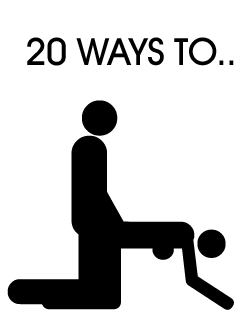
\includegraphics[width=2.5cm]{20waysto/f00.png}&

\includegraphics[width=2.5cm]{20waysto/f01.png}&

\includegraphics[width=2.5cm]{20waysto/f02.png}&
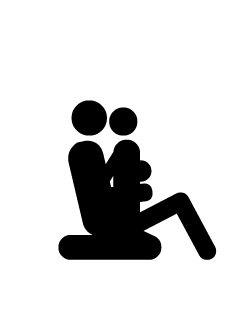
\includegraphics[width=2.5cm]{20waysto/f03.png}\\

\includegraphics[width=2.5cm]{20waysto/f10.png}&
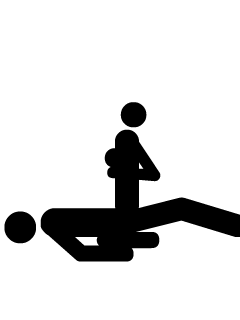
\includegraphics[width=2.5cm]{20waysto/f11.png}&

\includegraphics[width=2.5cm]{20waysto/f12.png}&
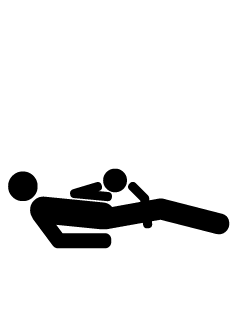
\includegraphics[width=2.5cm]{20waysto/f13.png}\\
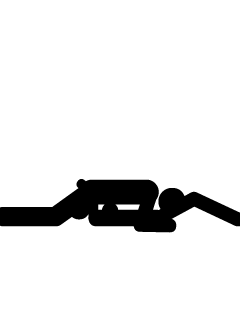
\includegraphics[width=2.5cm]{20waysto/f20.png}&

\includegraphics[width=2.5cm]{20waysto/f21.png}&

\includegraphics[width=2.5cm]{20waysto/f22.png}&
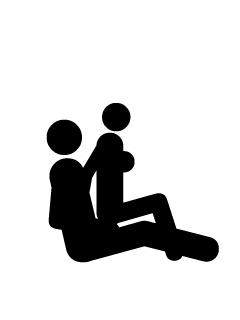
\includegraphics[width=2.5cm]{20waysto/f23.png}\\

\includegraphics[width=2.5cm]{20waysto/f30.png}&
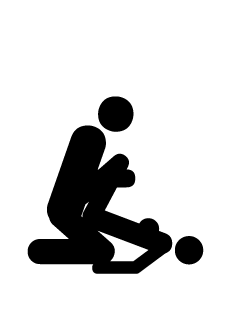
\includegraphics[width=2.5cm]{20waysto/f31.png}&
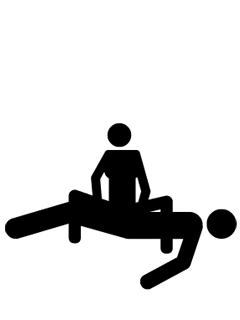
\includegraphics[width=2.5cm]{20waysto/f32.png}&

\includegraphics[width=2.5cm]{20waysto/f33.png}\\
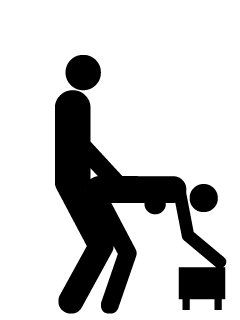
\includegraphics[width=2.5cm]{20waysto/f40.png}&
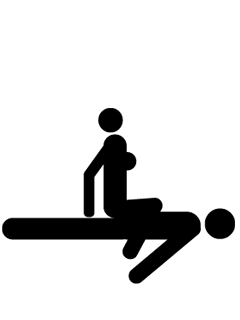
\includegraphics[width=2.5cm]{20waysto/f41.png}&

\includegraphics[width=2.5cm]{20waysto/f42.png}&

\includegraphics[width=2.5cm]{20waysto/f43.png}\\
\end{tabular}


%\includegraphics{20 ways to/Frame0.png}
	\caption{The figure for the Day spread of the Wager E09} \label{fig:20 ways}
\end{figure}

\begin{figure}
\input{E11}
\caption{This is the official Checklist for Wager E11} \label{fig:KamaSutra}
\end{figure}

\begin{figure}

\emph{The Great Roleplay Rumble}
\begin{itemize}
  \item Doctor-Patient
  \item Prostitute Client
  \item Zombie Zombie (rippable clothing)
  \item Zombie Survivor
  \item Teenagers in Slasher Fic
  \item Last couple alive
  \item Librarians
  \item Porno
  \item Plumber HouseWife
  \item Master Slave
  \item Boss Worker
  \item Pizza Delivery Guy 
  \item Ancient Communication Stones
  
\end{itemize}
\caption{This is the Listing for Wager E13} \label{fig:Roleplay}
\end{figure}
 \cleardoublepage
 %
 

 \section{Dares}

 \renewcommand{\theenumi}{\thesubsection.\arabic{enumi}}

   \subsection{Danielle Dares Sam}

\begin{enumerate}
\item  To stay up and watch the sun to rise with her and kiss her the moment its above the horizon.

\item  To go 2 Hours without making an innuendo, and if he manages to achieve such a feat, will receive fellatio.

\item  To meet her at an establishment pretending not to know her, and attempt to pick her up.

\item  To have a physical Poke war. 

\item  To dress in fitting historical costuming (Toga, Bulla, etc.) and read to her a translation of her favourite poems.  Assuming she can hold out  jumping on him, special reward ensues - must be completed to find out.  hehe 

\item  To sleep with her in her car, preferably during heavy rain (insert `very wet' joke here) 

\item To perform Cunnilingus, after consuming ananas Juice.

\item To To Allow her to lick Tabasco Sauce off of him.

\item To Allow her to lick wasabi off of him.

\end{enumerate}

 

  \subsection{Sam Dares Danielle:}

\begin{enumerate}
\item  To sleep with him with Dynamite by Taio Cruz, playing in background .

\item  To go 2 Hours without Making any reference to history, and if she manages such a feet of the calibre of the labours of Hercules, will receive Cunnilingus. 

\item  To spend all possible time in a day With no clothes on

\item  To awaken Samuel via means of Fellatio.

\item  To Skinny-dip along with Sam in her pool.

\item  To wear her skirt 3 inches above her knee for a single day.

\item  To Do activities in Her car with Sam so that the windows fog, to a point where it is impossible to see from the outside in or the inside out.

\item  To Kiss him in the rain.

\item To attempt an underwater blowjob.

\end{enumerate}

 
 \cleardoublepage
 %\section{Complex Numbers}
\begin{align}
z &= a+ib \hfill a,b \in \mathbb{R}\\
z&=4 \text{ Purely Real}\\
z&=2i \text{ Purely Imaginary}\\
\hline\\
\text{if } z &= -5i+2\\
\Re(z) &= 2\\
\Im(z) &= -5\\
\text{if } w &= 1-i\\
zw &= (-5i+2)(1-i)\\
&= -5i+2-2i+5i^2\\
&= -5i-2i+2-5\\
&= -7i-3\\
\hline
z&= r(\cos(\theta) + i \sin(\theta)) \text{ polar form}\\
r&= |z| = \text{modulus of }z\\
\arg{z} &= \tan^{-1}{\frac{\Re(z)}{\Im(z)}}
\end{align}
 

  

 


 



 

 \textbf{\textit{ Signed  }}

 \textbf{X\_\_Samuel\_Carter\_\_\_\_\_\_  }

 \textbf{X\_\_Danielle\_Jackson\_\_\_  }

 

 


\end{document}



